\chapter{Embedding Top-Down Join Enumerator}
\label{topdownint}
In this chapter we propose a new method of doing join enumeration in transformation-based optimizers based on ideas from memoization based join enumerators. DP-based and memoization-based enumeration algorithms\cite{fender2011new,fender2012effective,fender2013top} for join enumeration are more efficient in comparison to transformation-based ones in that they are able to enumerate the entire space without generating duplicates. 
In Section 6.1 we describe the algorithm, Section 6.2 describes the process for logical space generation and in  
Section 6.3 we describe a scheme for combining the two. 

\section{Conservative Partitioning}
\label{conservativePartitioning}
We describe in greater detail the conservative partitioning algorithm, denoted by \textsc{MinCutConservative} given by Pit Fender et al.\cite{fender2012effective}. The conservative partitioning algorithm is used in graph based join enumeration algorithm \textsc{TDMinCutConservative}. We try to use it here in a transformation based setting. \\

The algorithm emits all ccps for a connected vertex set $S \subseteq V$ where V is the vertex set of the query graph G=(V,E). The basic idea of conservative partitioning is to successively enhance a connected set C by members of its neighbourhood $N(C)$ at every recursive iteration. The process starts with a single vertex $t \in S$ through a redefinition of $N(\phi) = {t}$. This way, we ensure that at every instance of the algorithm's execution $C$ is connected. Since $S$ and $C \subset S$ are connected, for every possible complement $S \setminus C$ there must exist a join edge $(v1, v2)$, where $v1 \in C$ and $v2 \in (S \setminus C)$ holds. If at some point of enlarging $C$ its complement $S \setminus C$ in S is connected as well, the algorithm has found a ccp for S. \\

\begin{figure}[here]
\begin{center}
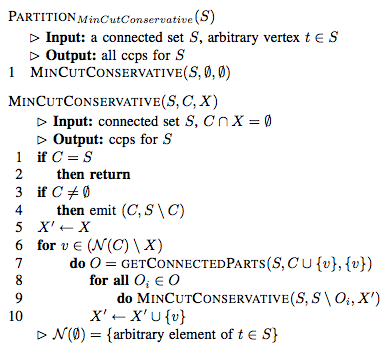
\includegraphics[width=9cm]{Figures/mincutconservative.png}
\end{center}
\caption{Pseudocode for \textsc{MinCutConservative}}
\label{fig:mincutconservative}
\end{figure}

\textsc{MinCutConservative} performs well even on when star queries are considered, where constructing every possible connected subset C of S produces an exponential overhead because most of the complements $S \setminus C$ are not connected and the partitions $(C, S \setminus C)$ computed this way are not valid ccps. Since the set C is expanded conservatively, this method remains effective. For pseudocode of the algorithm see Figure \ref{fig:mincutconservative}.

\section{Using Graph based enumeration}
We replace the existing join enumeration rules for commutativity and left associativity with a new  \textsc{N-ary Join} rule. The \textsc{N-ary Join} rule generates all ccps for the given set of n-relations. It is in essence a vanilla coated \textsc{MinCutConservative} algorithm.

\begin{defn}
A base equivalence class is defined as an equivalence class which is either a base relation or has atleast one  child logical operation node which is not a join operator.
\end{defn}

To run the \textsc{MinCutConservative} algorithm, we need the join graph induced by the base equivalence classes. For this we store two additional sets at each equivalence node:

\begin{itemize}
	\item \textsc{EqSet} : A set of all combinations of base equivalence classes being joined to generate this equivalence class. Along with this we need to store the ids of join operators of a feasible join ordering for these base equivalence class. This is used to infer the join graph.
	\item \textsc{HSet} : A set of hashes. For every set of base equivalence class that we enumerate, we generate a hash and store it in the parent equivalence class as a proof that this set has been enumerated. This is to prevent repeated enumeration of the same set of base equivalence classes.
\end{itemize}

Given with the above information, when \textsc{N-ary Join} rule is applied at a logical join operator $op$ get the \textsc{EqSet} of the left child and right child. For all combination of $S=S_{1} \cup S_{2}$ where $S_{1}\in \textsc{EqSet}_{L}$ and $S_{2}\in \textsc{EqSet}_{R}$, generate $hash(S)$ and check to ensure it has not been enumerated before. It it has not been enumerated, call \textsc{MinCutConservative}$(G_{|S})$. For every ccp generated add a new operation node to $child(parent(op))$. For every new equivalence class generated, insert it as a left-deep tree got by doing a depth-first traversal on the join graph (such a tree exists as the graph induced by these base equivalence classes is connected).
